% --------------------------------------
% Document Class
% --------------------------------------
\documentclass[a4paper,11pt]{article}
% --------------------------------------



% --------------------------------------
% Use Package
% --------------------------------------


\usepackage[francais]{babel}
%\usepackage{ucs}
\usepackage[utf8]{inputenc}
\usepackage[T1]{fontenc}

\usepackage{makeidx}
\usepackage{color}
\usepackage{graphicx}
\usepackage{float}
\usepackage[hidelinks]{hyperref} 
\usepackage{geometry}
%\usepackage{lastpage}
%\usepackage{marginnote}
\usepackage{fancyhdr}
%\usepackage{titlesec}
%\usepackage{framed}
\usepackage{amsmath}
\usepackage{empheq}
\usepackage{array}
\usepackage{multicol}
%\usepackage{adjustbox}

% insert code
\usepackage{listings}

% define our color
\usepackage{xcolor}

% code color
\definecolor{ligthyellow}{RGB}{250,247,220}
\definecolor{darkblue}{RGB}{5,10,85}
\definecolor{ligthblue}{RGB}{1,147,128}
\definecolor{darkgreen}{RGB}{8,120,51}
\definecolor{darkred}{RGB}{160,0,0}

% other color
\definecolor{ivi}{RGB}{141,107,185}


\lstset{
  language=Scilab,
  captionpos=b,
  extendedchars=true,
  frame=lines,
  numbers=left,
  numberstyle=\tiny,
  numbersep=5pt,
  keepspaces=true,
  breaklines=true,
  showspaces=false,
  showstringspaces=false,
  breakatwhitespace=false,
  stepnumber=1,
  showtabs=false,
  tabsize=3,
  basicstyle=\small\ttfamily,
  backgroundcolor=\color{ligthyellow},
  keywordstyle=\color{ligthblue},
  morekeywords={include, printf, uchar},
  identifierstyle=\color{darkblue},
  commentstyle=\color{darkgreen},
  stringstyle=\color{darkred},
}


% --------------------------------------



% --------------------------------------
% Page setting
% --------------------------------------
%\pagestyle{empty}
\setlength{\headheight}{15pt}

\setcounter{secnumdepth}{3}
\setcounter{tocdepth}{2}

\makeatletter
\@addtoreset{chapter}{part}
\makeatother 

\hypersetup{         % parametrage des hyperliens
  colorlinks=true,      % colorise les liens
  breaklinks=true,      % permet les retours à la ligne pour les liens trop longs
  urlcolor= blue,       % couleur des hyperliens
  linkcolor= black,     % couleur des liens internes aux documents (index, figures, tableaux, equations,...)
  citecolor= green      % couleur des liens vers les references bibliographiques
}

% --------------------------------------

% --------------------------------------
% Information
% --------------------------------------
\title{Compte-rendu TP8 Rdf : Classifcation non supervisée}
\author{Elliot VANEGUE et Gaëtan DEFLANDRE}
% --------------------------------------

\definecolor{myColor}{rgb}{0.5, 0.1, 0.75}

% --------------------------------------
% Begin content
% --------------------------------------
\begin{document}
  
  % Set language to english
  \selectlanguage{francais}
  
  % Start the page counting
  \pagenumbering{arabic}
  
  \maketitle
  
  \mbox{}
  \newpage
  \clearpage
  
  \section*{Introduction}
  Jusque là nous avons vu des méthodes de classification supervisée, c'est à dire qu'elles produisaient
  des règle automatiquement à partir de données fournit au préalable. 
  Lors de ce TP, nous allons voir une méthode non supervisée qui est la méthode du K-means. Cette méthode
  va permettre de séparer les données de l'image en plusieurs groupe sans fournir de base données. Nous allons
  nous servir de cette technique afin de trouver le seuil le plus approprié à la binarisation d'une image.
  
  \section{Classification des données Iris par la méthode K-means}
  Dans un premier temps, nous classifions les données Iris en trois classes représentant les trois espèces
  d'iris. Pour différencier les iris nous avons quatre caractéristiques fournit dans les données : la largeur et
  la longueur du séparle et la largeur et la hauteur du pétale.\\
  
  \begin{figure}[H]
    \center
    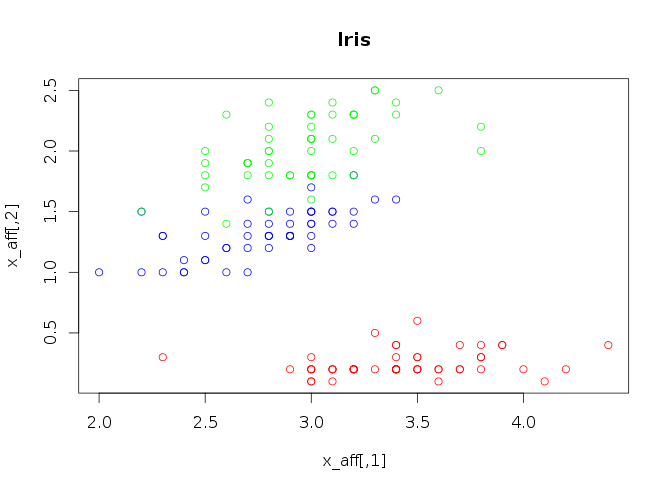
\includegraphics[width=9cm]{resultat/separation_espece.png}
    \caption{Graphique de séparation des données des trois espèces d'iris}
  \end{figure}
  
  Nous appliquons la classification K-means sur ces données afin de voir si celui-ci sépare correctement les données.
  Le principe de l'algorithme du K-means est de minimiser la distance entre le centre d'une classe et les données
  qui la constitue. Pour cela, ces centres sont le plus éloigné entre eux à la première itération, puis ils se 
  déplacent à chaque itération jusqu'à se retrouver au centre des données d'une classe.\\
  
  %TODO réfléchir à pourquoi on a des données qui ont deux formes
  Lorsque nous effectuons cette algorithme sur les données Iris avec quinze itérations, nous pouvons voir que l'un des centres se trouve 
  entre deux classes tandis que les deux autres se retrouvent sur la même classe.
  
  \begin{figure}[H]
    \center
    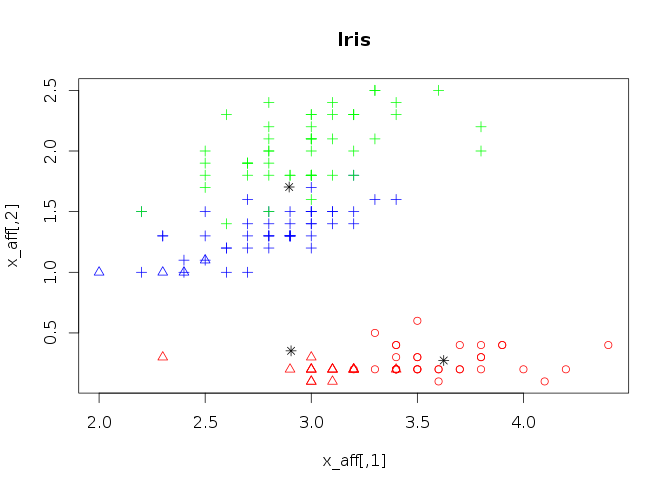
\includegraphics[width=9cm]{resultat/kmeans.png}
    \caption{Résultat de la classification des données Iris par K-means}
  \end{figure}
  
  Afin de détecter d'oû vienne les erreurs, nous avons répété le processus précédent cinq fois en y ajoutant
  une variable permettant de calculer les erreurs. Ainsi nous voyons que le centre se déplace est atteint une
  position permettant de bien séparer chaque classe. Voici un tableau comportant la position de chaque centre
  sur les cinq itération, ainsi que le taux d'erreur de la classification.\\
  
  \begin{center}
  \begin{tabular}{|c|c|c|c|c|}
    \hline
    iteration & centre 1 & centre 2 & centre 3 & taux d'erreur\\
    \hline
    1 & (5.17 , 3.62) & (4.73 , 2.90) & (6.31 , 2.89) & 0.33\\
    \hline
    2 & (5.90 , 2.74) & (5.00 , 3.42) & (6.85 , 3.07) & 0.10\\
    \hline
    3 & (5.00 , 3.42) & (5.90 , 2.74) & (6.85 , 3.07) & 0.10\\
    \hline
    4 & (4.73 , 2.90) & (6.31 , 2.89) & (5.17 , 3.62) & 0.33\\
    \hline
    5 & (6.85 , 3.07) & (5.90 , 2.74) & (5.00 , 3.42) & 0.10\\
    \hline
  \end{tabular}
  \end{center}
  
  %la pas sur mais je vois pas quoi en conclure.
  On ne remarque pas de gros changement entre les itérations, à part pour le point 1 entre les itérations
  4 et 5. De plus, le taux d'erreur varie, mais il revient sur d'ancienne valeur, ce qui signifie que les 
  cinq itération que nous venons de réaliser ne servent pas et que les centres étaient proche de leur 
  état final.
  
  %TODO ajout de l'image après les 5 itérations
  
  %TODO faire la suite
  
  \section{Segmentation d'une image de textures par classification non supervisée des pixels}
  Maintenant nous allons segmenter l'image des gâteaux étudié lors du TP3 grâce à la classification
  K-means. Nous créons une matrice composé des données des deux images. Nous pouvons voir que le nuage
  de point est composé de deux forme distincte : l'une est à l'horizontale et relativement grosse, tandis 
  que l'autre est parfaitement à la verticale.
  
  \begin{figure}[H]
    \center
    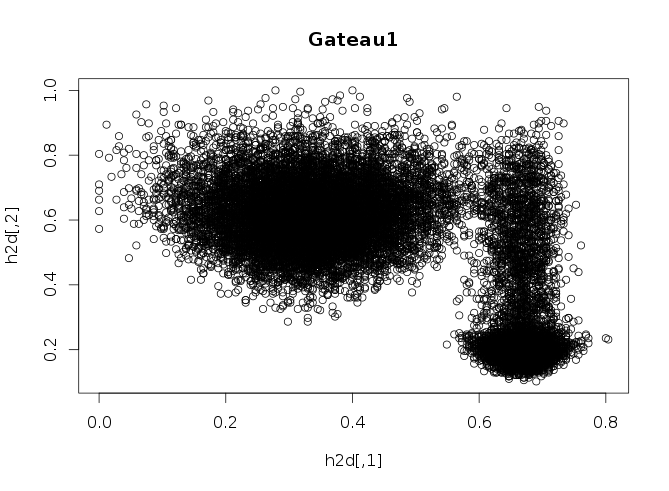
\includegraphics[width=9cm]{resultat/image_combine.png}
    \caption{Graphique des données des deux images de gâteaux}
  \end{figure}
  
  Nous effectuons la classification des données précédente avec K-means en 30 itération. Le résultat
  nous donne une classification diagonale avec comme premier centre le centre de la forme horizontale et 
  comme second centre le bas de la forme verticale. Cette algorithme n'a donc pas pris une classe par forme,
  mais à légèrement découpé la forme verticale.
  
  \begin{figure}[H]
    \center
    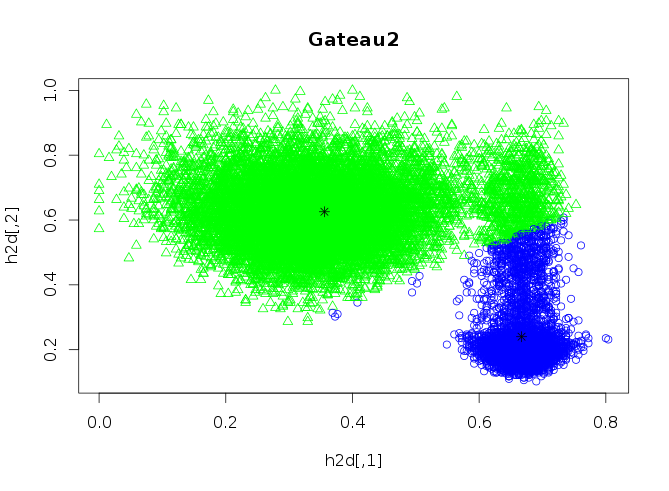
\includegraphics[width=9cm]{resultat/classification_gateau.png}
    \caption{Résultat de la classification de K-means des données des deux images de gâteaux}
  \end{figure}
  
  %TODO ajout des résultats
  
\end{document}  